\chapter{Конструкторская часть}

\section{Введение}
В данном разделе представлены схемы алгоритмов сортировок: блинной, поразрядной, бинарным деревом, а также их теоретическая оценка трудоемкости.

\section{Разработка алгоритмов}
В данном разделе представлены схемы алгоритмов для блинной сортировки (рисуноки \ref{img:pancake}, \ref{img:findMaxIndex} и \ref{img:flip}), алгоритма поразрядной сортировки (рисунки \ref{img:radix} и \ref{img:countSort}) и алгоритма сортировки бинарным деревом (рисунки \ref{img:treeSort} и \ref{img:tree}).

\begin{figure}[h]
	\centering
	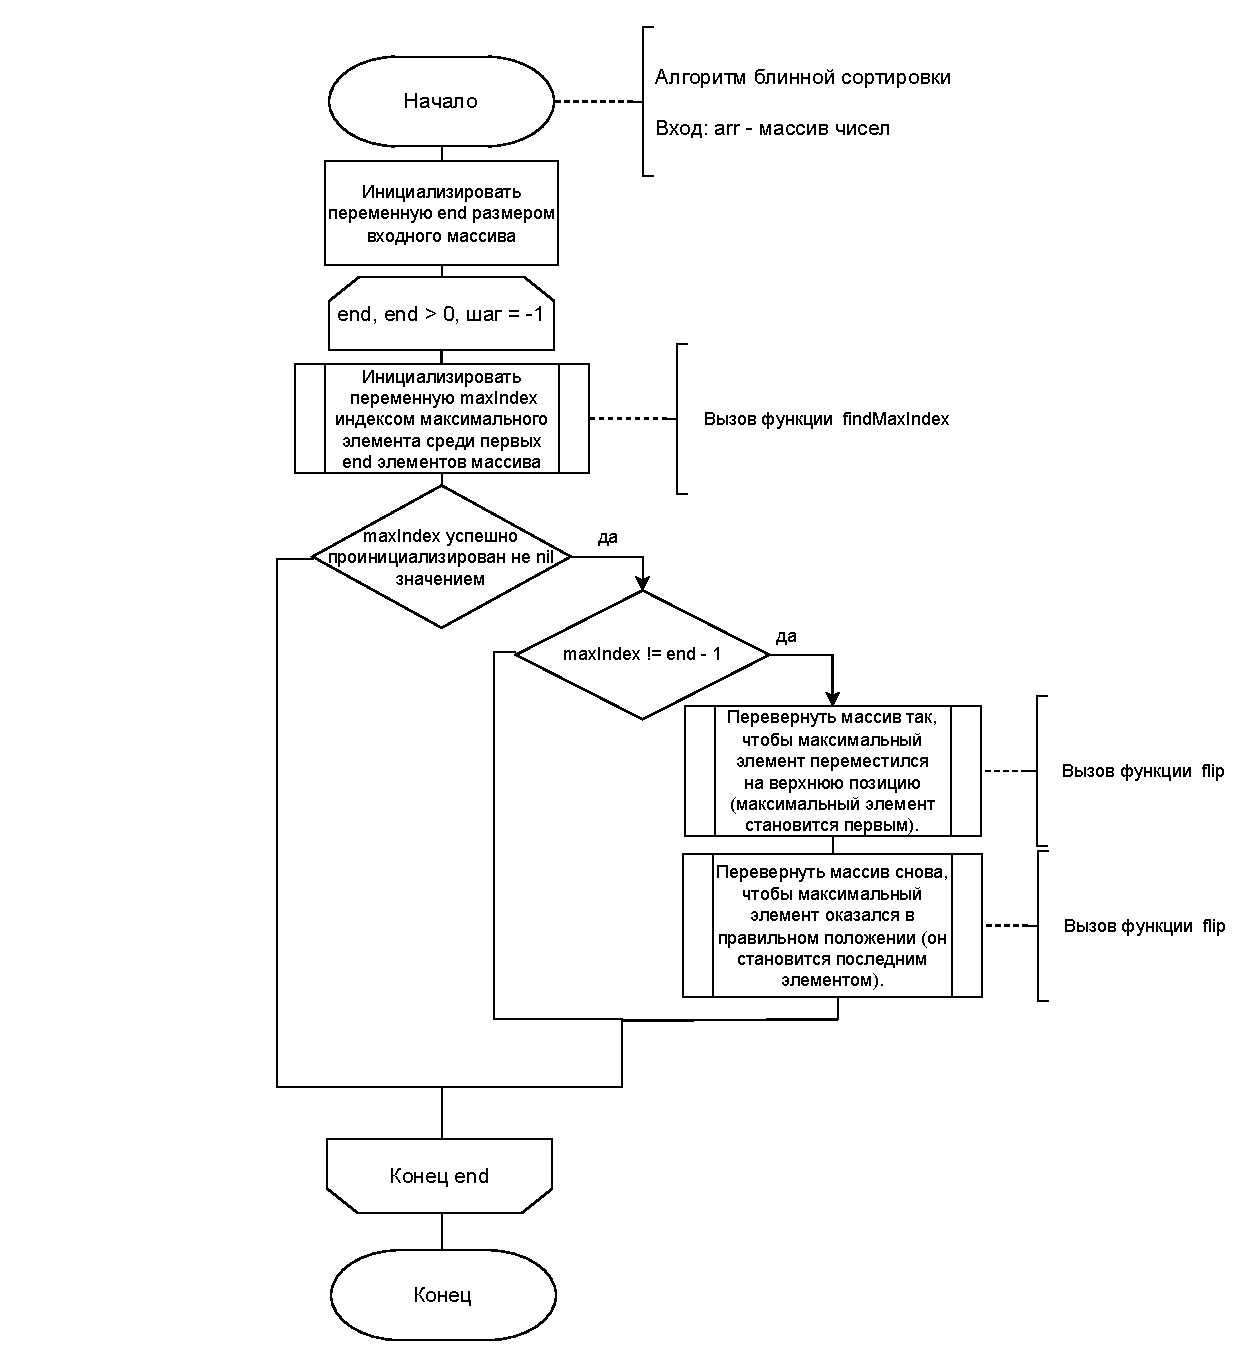
\includegraphics[width=1\linewidth]{img/pancake.pdf}
	\caption{Схема блинного алгоритма сортировки}
	\label{img:pancake}
\end{figure}

\begin{figure}[h]
	\centering
	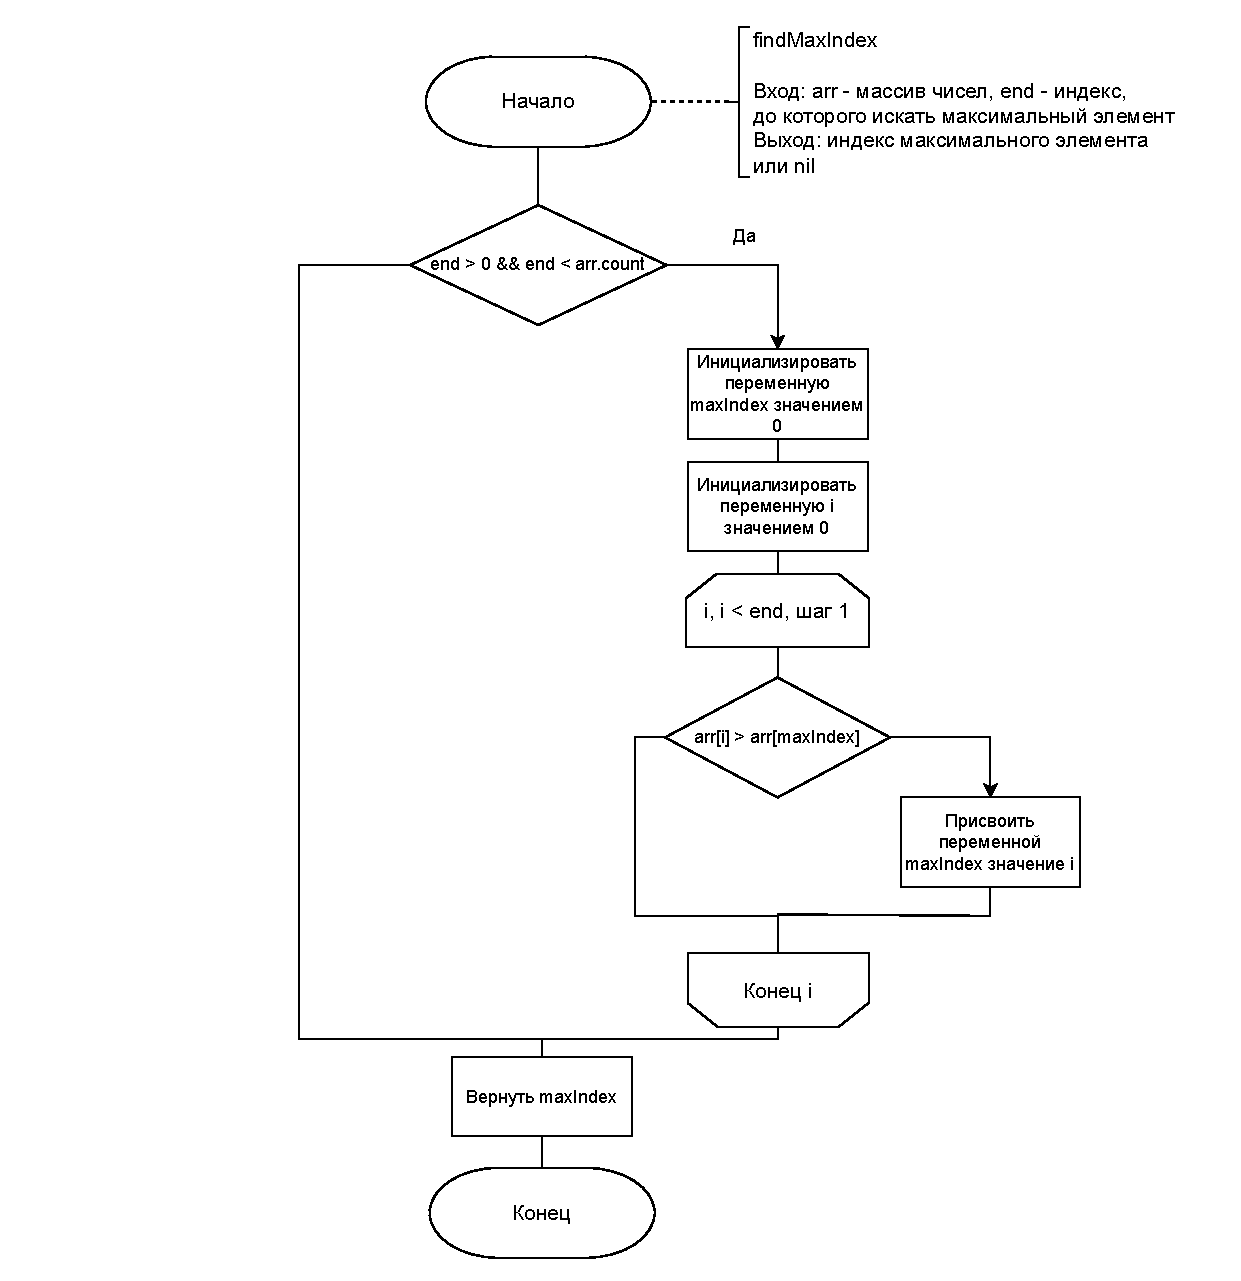
\includegraphics[width=1\linewidth]{img/findMaxIndex.pdf}
	\caption{Схема алгоритма поиска индекса максимального элемента}
	\label{img:findMaxIndex}
\end{figure}

\begin{figure}[h]
	\centering
	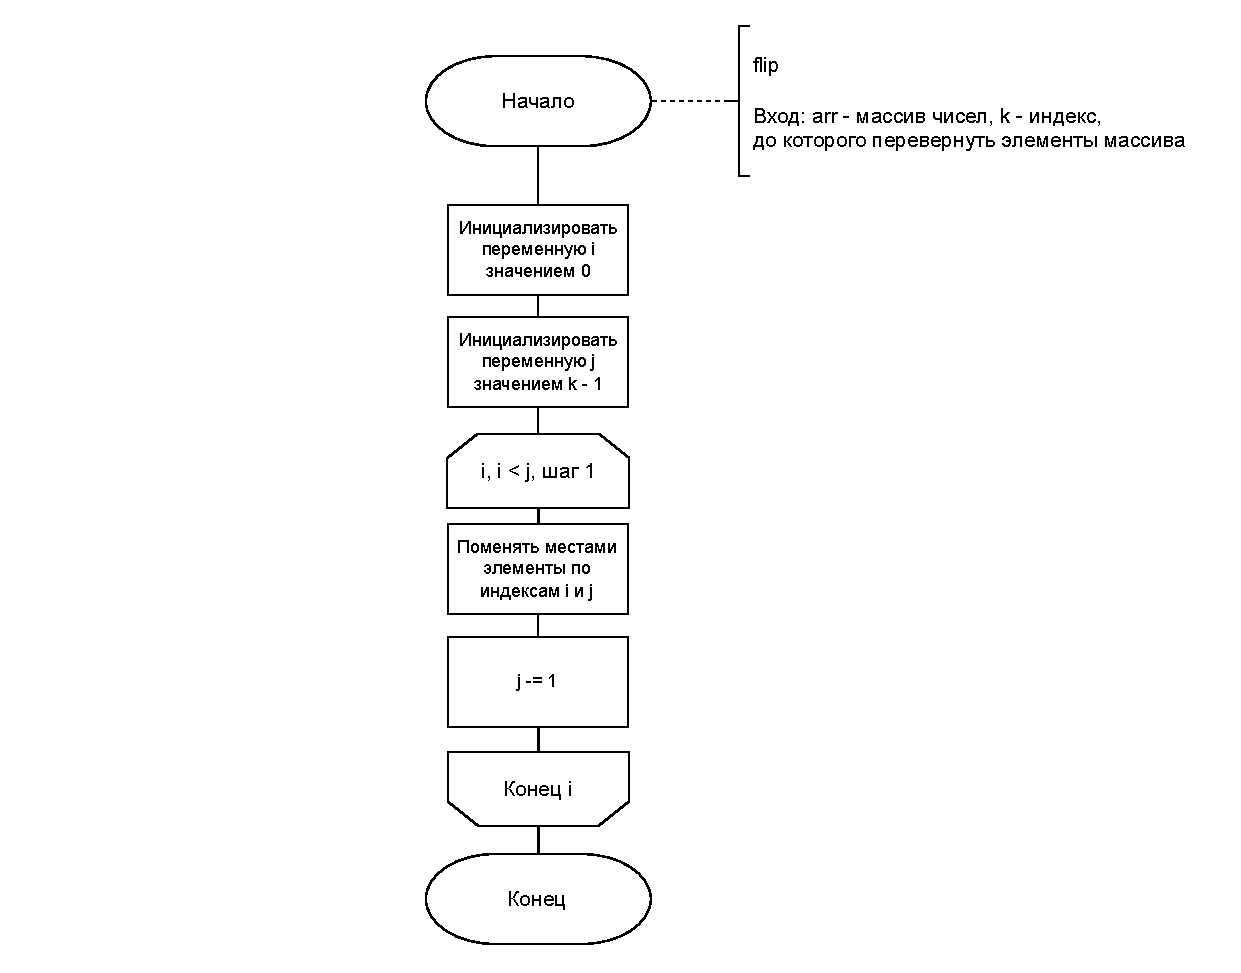
\includegraphics[width=1\linewidth]{img/flip.pdf}
	\caption{Схема алгоритма переворачивания массива}
	\label{img:flip}
\end{figure}

\begin{figure}[h]
	\centering
	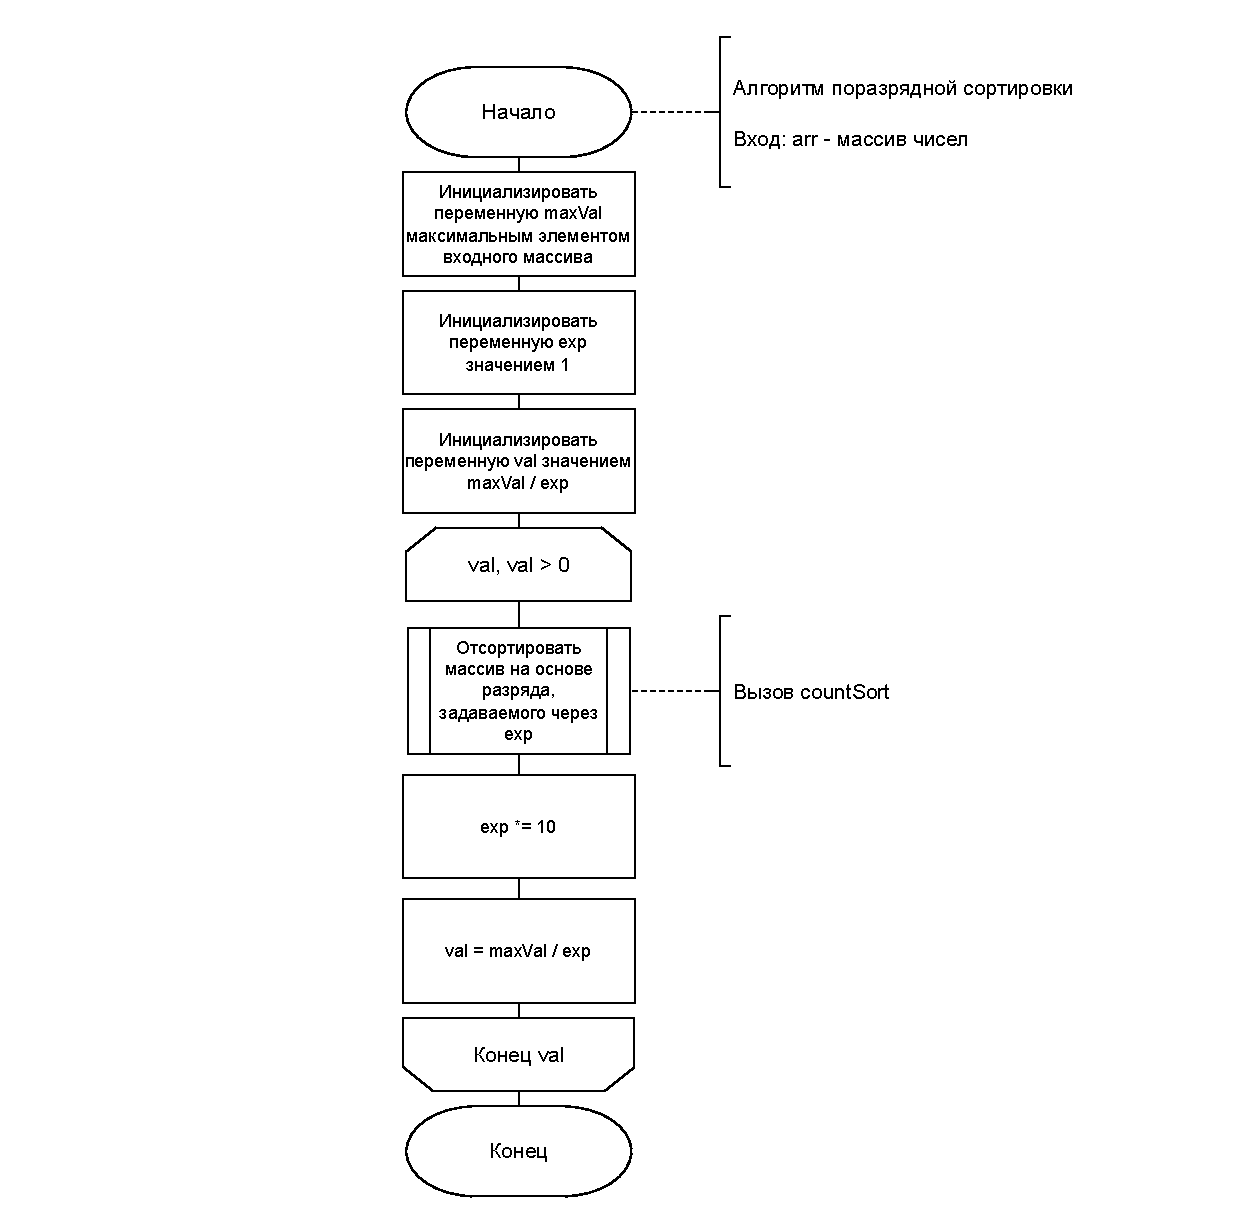
\includegraphics[width=1\linewidth]{img/radix.pdf}
	\caption{Схема поразрядного алгоритма сортировки}
	\label{img:radix}
\end{figure}

\begin{figure}[h]
	\centering
	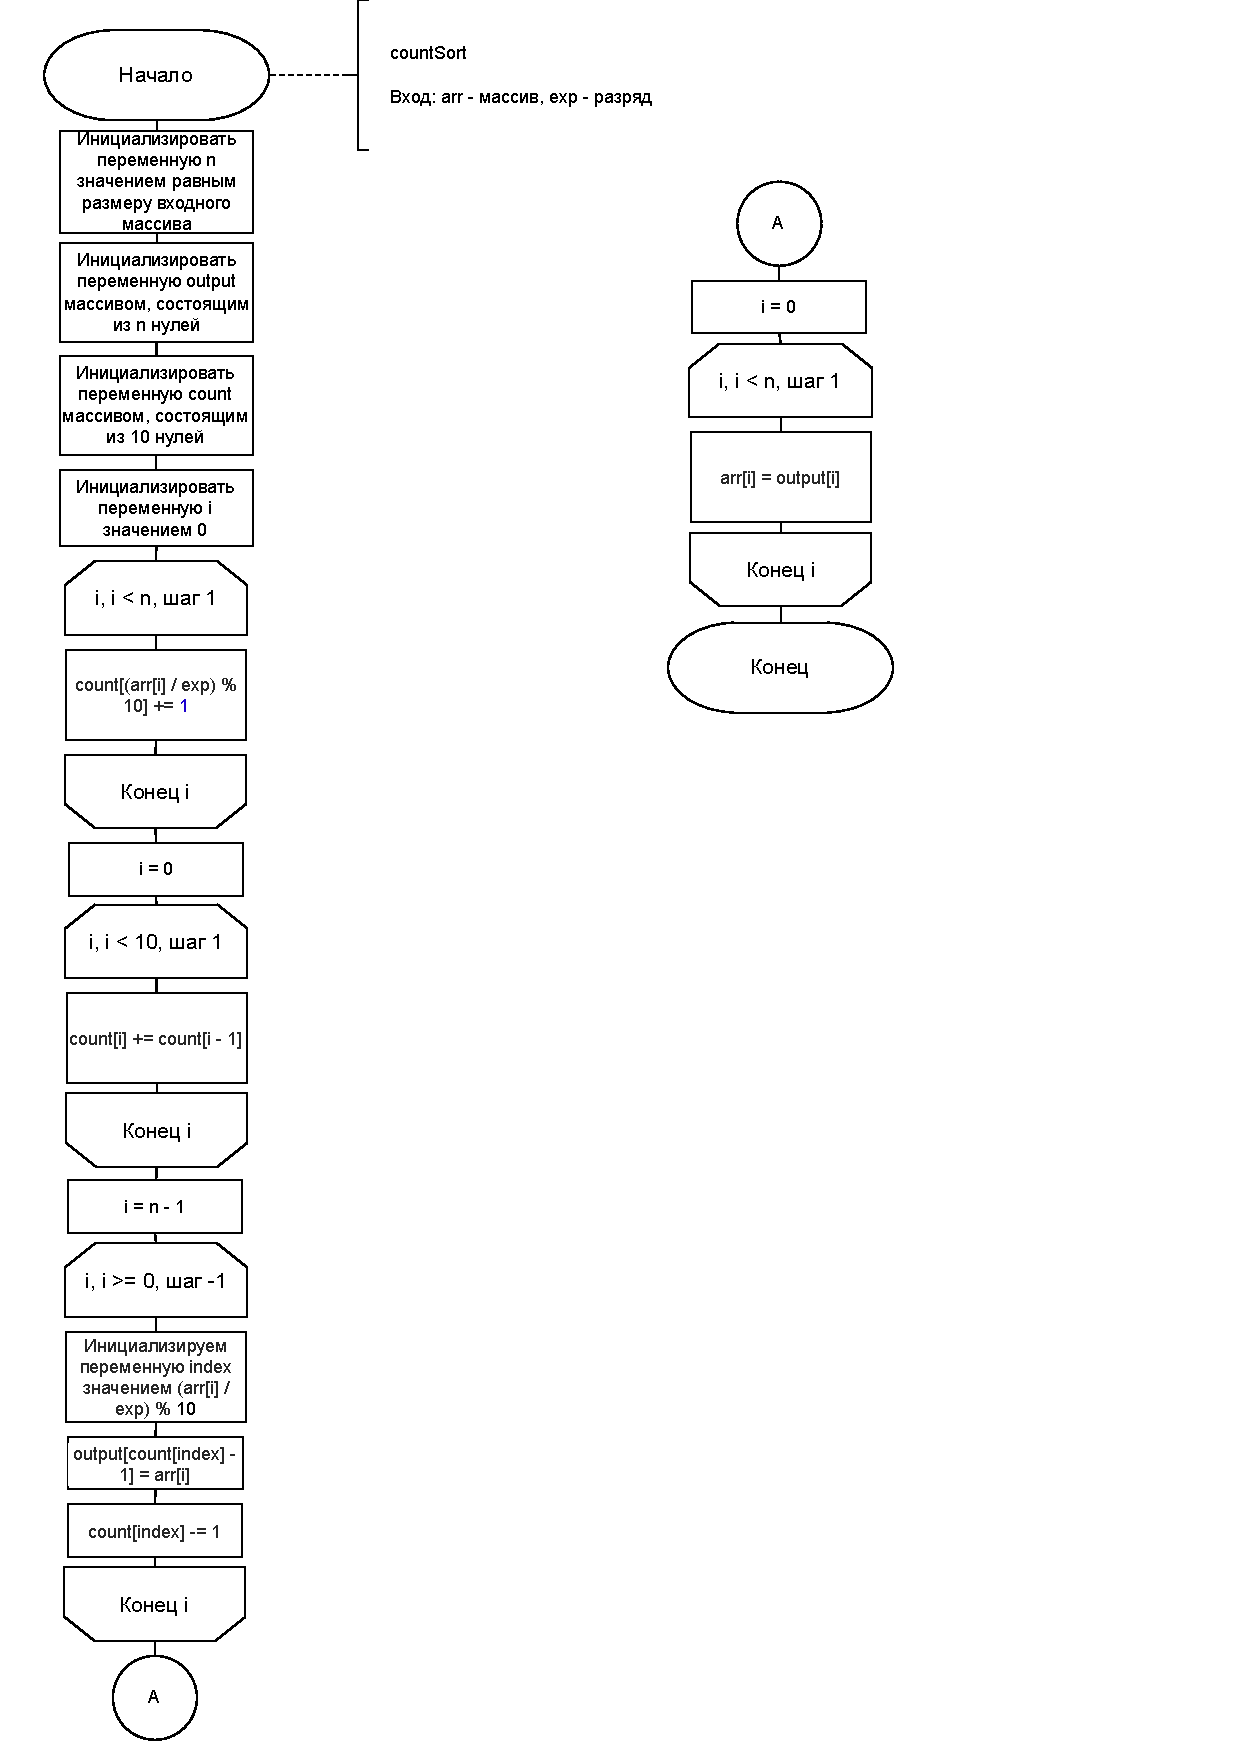
\includegraphics[width=1\linewidth]{img/countSort.pdf}
	\caption{Схема алгоритма сортировки подсчетом}
	\label{img:countSort}
\end{figure}

\begin{figure}[h]
	\centering
	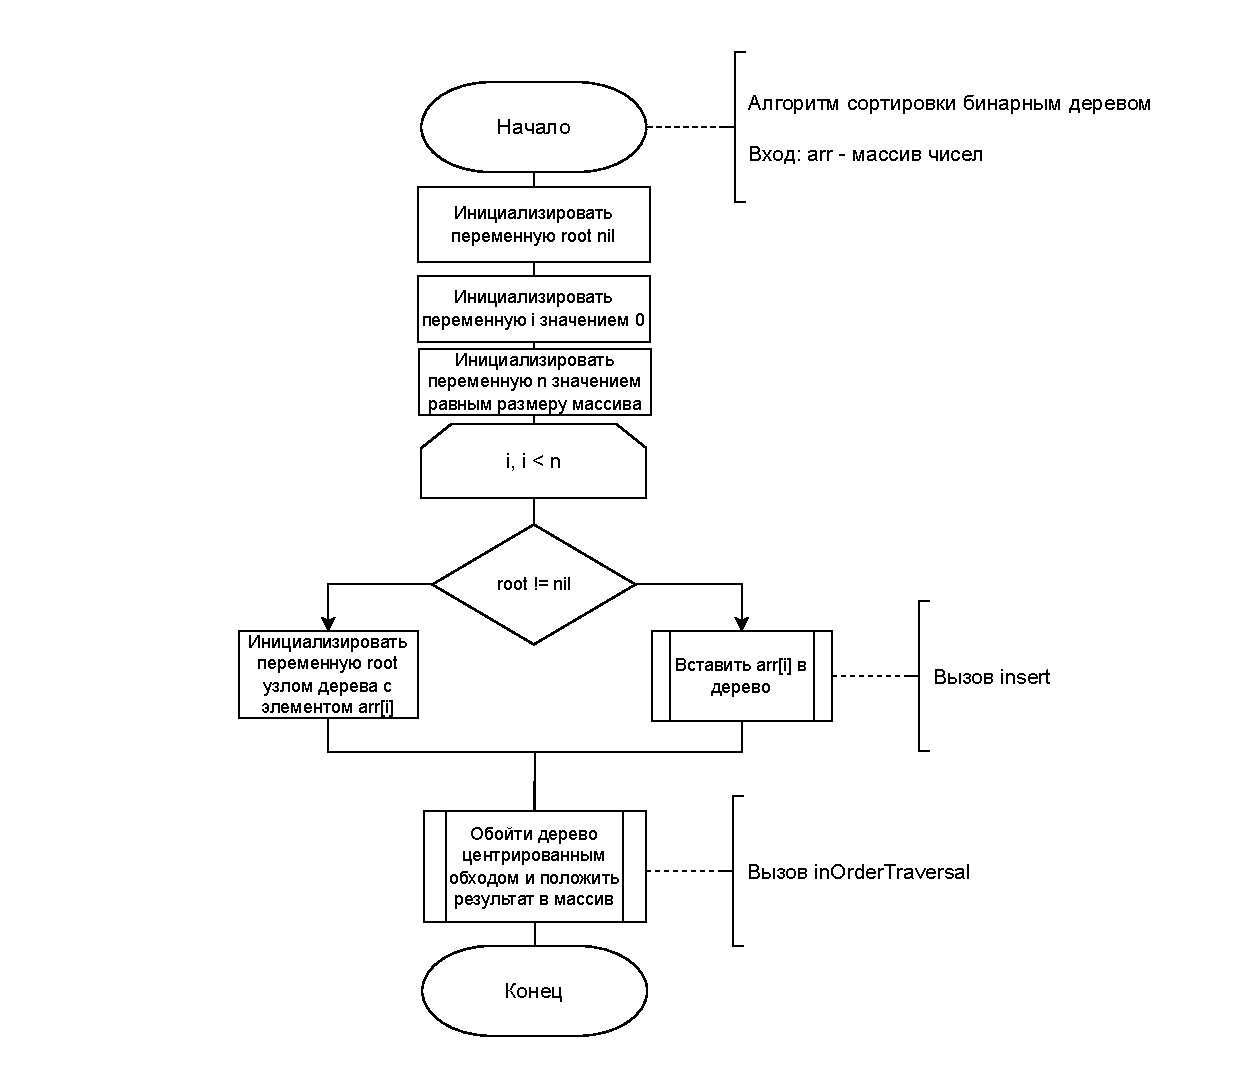
\includegraphics[width=1\linewidth]{img/treeSort.pdf}
	\caption{Схема алгоритма сортировки бинарным деревом}
	\label{img:treeSort}
\end{figure}

\begin{figure}[h]
	\centering
	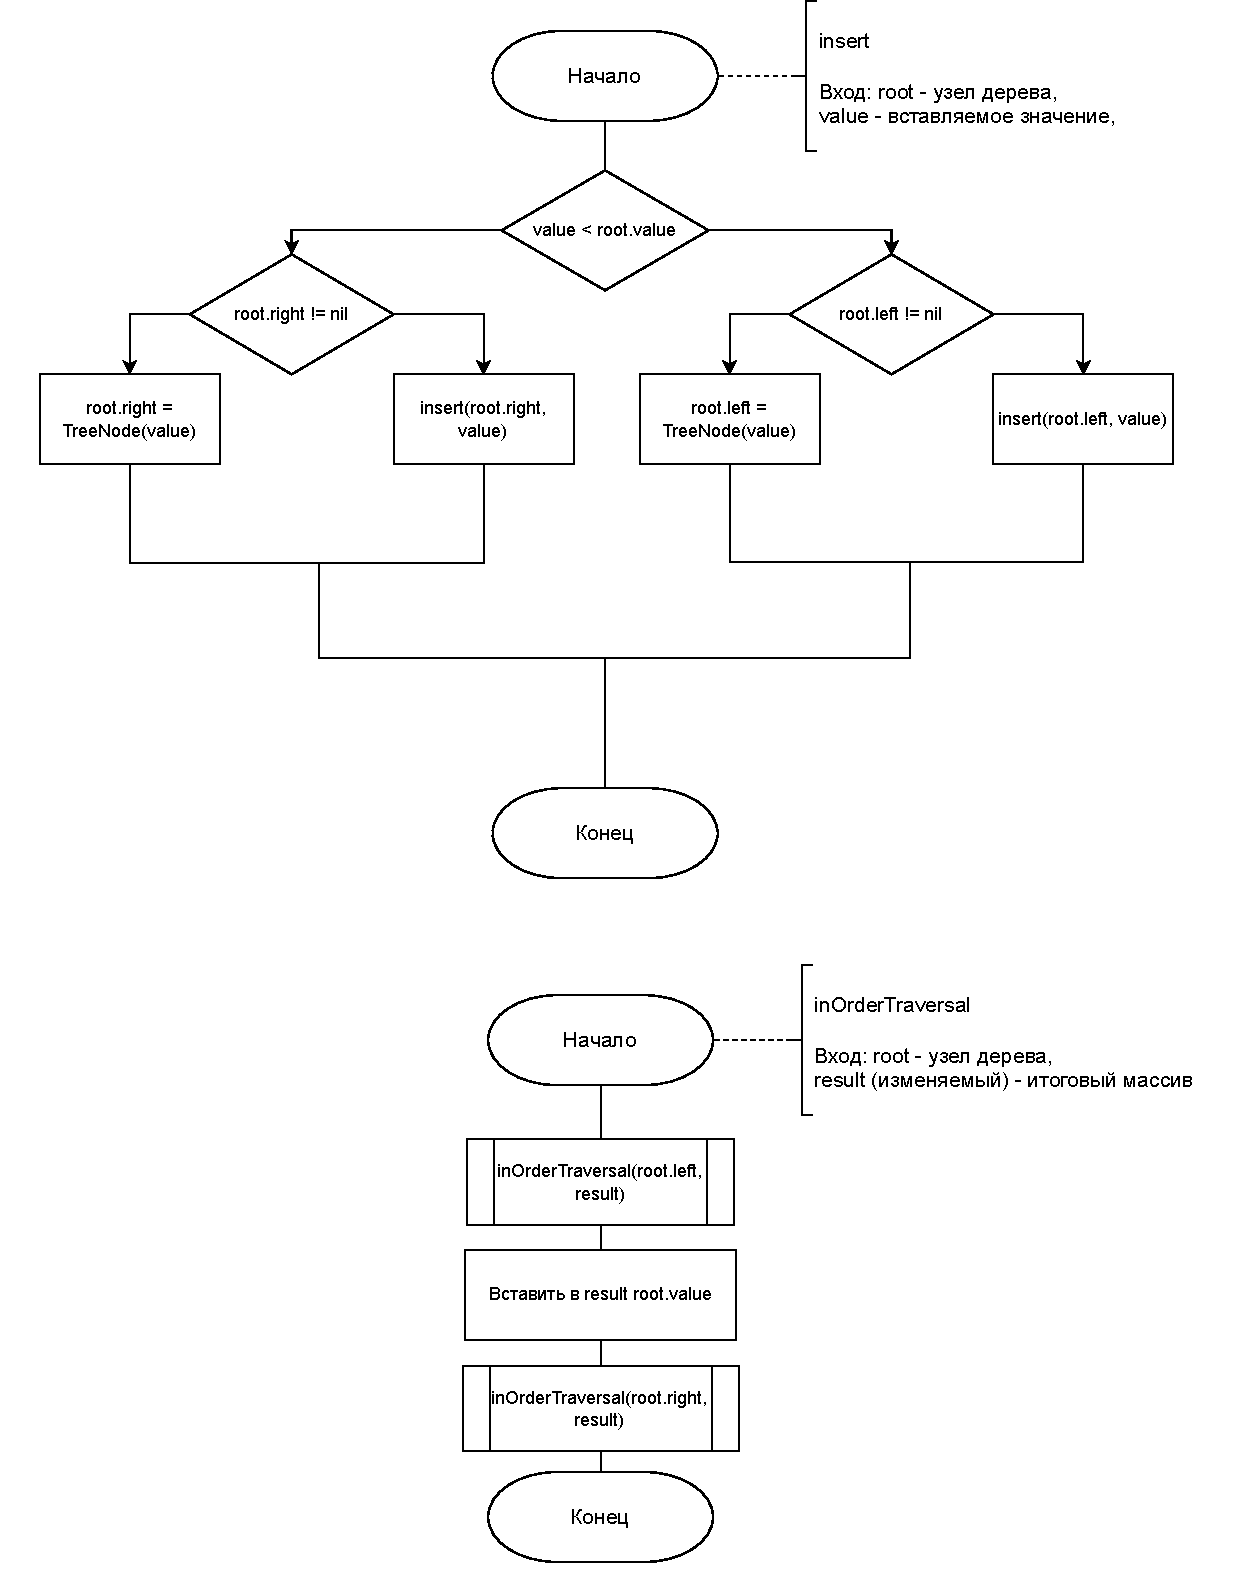
\includegraphics[width=1\linewidth]{img/tree.pdf}
	\caption{Схема методов работы с деревом}
	\label{img:tree}
\end{figure}
\clearpage

\section{Модель вычислений для проведения оценки трудоемкости}

Введем модель вычислений, которая потребуется для определения трудоемкости каждого отдельного взятого алгоритма умножения матриц.
\begin{enumerate}[label={\arabic*)}]
	\item Трудоемкость базовых операций имеет:
	\begin{itemize}[label=---]
		\item равную 1:
		\begin{equation}
			\label{for:operations_1}
			\begin{gathered}
				+, -, =, +=, -=, ==, !=, <, >, <=, >=, [], ++, {-}-,\\
				\&\&, >>, <<, ||, \&, |
			\end{gathered}
		\end{equation}
		\item равную 2:
		\begin{equation}
			\label{for:operations_2}
			*, /, \%, *=, /=, \%=
		\end{equation}
	\end{itemize}
	\item Трудоемкость условного оператора:
	\begin{equation}
		\label{for:if}
		f_{if} = f_{\text{условия}} + 
		\begin{cases}
			min(f_1, f_2), & \text{лучший случай}\\
			max(f_1, f_2), & \text{худший случай}
		\end{cases}
	\end{equation}
	\item Трудоемкость цикла:
	\begin{equation}
		\label{for:for}
		\begin{gathered}
			f_{for} = f_{\text{инициализация}} + f_{\text{сравнения}} + M_{\text{итераций}} \cdot (f_{\text{тело}} +\\
			+ f_{\text{инкремент}} + f_{\text{сравнения}})
		\end{gathered}
	\end{equation}
	\item Трудоемкость передачи параметра в функции и возврат из функции равны 0.
\end{enumerate}

\section{Трудоемкость алгоритмов}

Была рассчитана трудоемкость алгоритмов сортировки.

\subsection{Блинная сортировка}

Для алгоритма блинной сортировки трудоемкость будет равна трудоемкости цикла по $end \in [1 \ldots N]$.

Трудоемкость цикла указана в формуле (\ref{complexity:pancake_main}).

\begin{equation}
	\label{complexity:pancake_main}
	f_{body} = 2 + N \cdot (f_{findMaxIndex} + %TODO: Переделать не под тело
	\begin{cases}
		2, \\
		2 + 2 \cdot f_{flip} 
	\end{cases}
	+ 1
	)
\end{equation}

Вычислим трудоемкость функции findMaxIndex. Результат представлен в формуле (\ref{complexity:findMaxIndex}).
\begin{equation}
	\label{complexity:findMaxIndex}
	f_{findMaxIndex} = 3 + 1 + 2 + end \cdot (2 +
		\begin{cases}
			3, \\
			3 + 1
		\end{cases}
	)
\end{equation}

Трудоемкость функции flip представлена в формуле (\ref{complexity:flip}).
\begin{equation}
	\label{complexity:flip}
	f_{flip} = 1 + 2 + 1 + end \cdot (1 + 3 + 2) = 4 + 6 \cdot end
\end{equation}

Таким образом, трудоемкость блинной сортировки в лучшем случае равна, формула (\ref{complexity:pancake_best}).
\begin{equation}
	\label{complexity:pancake_best}
	f_{best} = 2 + N \cdot 9 + \frac{1 + N}{2} \cdot N \cdot 5 = 2.5N^2 + 11.5N + 2 \approx 2.5N^2
\end{equation}

Трудоемкость в худшем случае представлена в формуле (\ref{complexity:pancake_worst}).
\begin{equation}
	\label{complexity:pancake_worst}
	f_{worst} = 2 + N \cdot 17 + \frac{1 + N}{2} \cdot N \cdot (6 + 2 \cdot 6) = 9N^2 + 26N + 2 \approx 9N^2 
\end{equation}

\clearpage

\subsection{Поразрядная сортировка}

Чтобы вычислить трудоемкость алгоритма поразрядной сортировки, нужно учесть следующее:

\begin{itemize}[label=---]
	
	\item функцию получения максимального элемента массива, трудоемкость которой указана в формуле~(\ref{сomplexity:get_max});
	\begin{equation}
		\label{сomplexity:get_max}
		f_{getMax} = 2 + 2 + N \cdot (2 + 
		\begin{cases}
			1, \\
			2
		\end{cases}
		)
	\end{equation}

	\item сортировку подсчетом, которая учитывает разряд, трудоемкость которой указана в формуле~(\ref{сomplexity:count_sort});
	\begin{equation}
		\label{сomplexity:count_sort}
		\begin{gathered}
			f_{countSort} = 2 + N + 10 + 2 + N \cdot (1 + 2 + 2 + 1 + 1 + 2) +\\
			+ 2 + 9 \cdot 6 + 2 + N \cdot (1 + 1 + 2 + 2 + 3 + 2 + 2 + 2) + \\
			+ 2 + N \cdot 5 = N \cdot (9 + 15 + 5) + 14 + 58 + 2 = 29N + 74
		\end{gathered}
	\end{equation}

	\item внешний цикл, в теле которого сортировка подсчетом, трудоемкость которого указана в формуле~(\ref{сomplexity:while});
	
	\begin{equation}
		\label{сomplexity:while}
		\begin{gathered}
			f_{while} = 2 + K \cdot (f_{countSort} + 2 + 2) = 2 + K \cdot (29N + 78) = \\
			29KN + 78K + 2
		\end{gathered}
	\end{equation}
\end{itemize}


В итоге, трудоемкость поразрядной сортировки равна:
\begin{equation}
	\label{complexity:radixSort}
	f_{radixSort} = 1 + 4 + 4N + 29KN + 78K + 2 = 29KN + 78K + 4N + 7
\end{equation}

\subsection{Сортировка бинарным деревом}
Трудоёмкость данного алгоритма посчитаем следующим образом: сортировка -- преобразование массива или списка в бинарное дерево поиска посредством операции вставки нового элемента в бинарное дерево.
Операция вставки в бинарное дерево имеет сложность $ \log_{2}(size)$, где $size$ - количество элементов в дереве.
Для преобразования массива или списка размером $size$ потребуется использовать операцию вставки в биннарное дерево $size$ раз, таким образом, итоговая трудоёмкость данной сортировки будет равна (\ref{for:binary_sort_perf}):
\begin{align}
\begin{split}
	\label{for:binary_sort_perf}
	f_{radix} &= size \cdot \log_{2}(size)
\end{split}
\end{align}

\section*{Вывод}
В данном разделе были представлены схемы алгоритмов сортировки и проведена теоретическая оценка трудоемкости алгоритмов. 
Результаты показывают, что поразрядная сортировка наиболее эффективна, а блинная сортировка - наименее эффективна.